\documentclass[tikz,border=10pt]{standalone}
% Shared look for every TikZ diagram. Load with % Shared look for every TikZ diagram. Load with % Shared look for every TikZ diagram. Load with \input{../../tools/tikz-style.tex}
\usepackage[T1]{fontenc}
\usepackage{lmodern}
\renewcommand{\sfdefault}{lmr}  % diagrams use the same serif as the text
\usetikzlibrary{arrows.meta, positioning, shapes.geometric, calc, fit, backgrounds}
\definecolor{cblue}{HTML}{4C78A8}
\definecolor{corange}{HTML}{F58518}
\definecolor{cgreen}{HTML}{54A24B}
\definecolor{cred}{HTML}{E45756}
\definecolor{cpurple}{HTML}{B279A2}
\definecolor{cgrey}{HTML}{6B6B6B}
\tikzset{
  every picture/.style={font=\sffamily, line width=1.2pt},
  box/.style={draw=#1, fill=#1!12, rounded corners=4pt, align=center, inner sep=7pt, minimum height=1.1cm},
  box/.default=cgrey,
  arrow/.style={-{Stealth[length=3mm]}, draw=cgrey, line width=1.4pt},
  title/.style={font=\sffamily\bfseries\Large},
  note/.style={font=\sffamily\small, text=cgrey, align=center},
}
\AtBeginDocument{\hyphenpenalty=10000 \exhyphenpenalty=10000}

\usepackage[T1]{fontenc}
\usepackage{lmodern}
\renewcommand{\sfdefault}{lmr}  % diagrams use the same serif as the text
\usetikzlibrary{arrows.meta, positioning, shapes.geometric, calc, fit, backgrounds}
\definecolor{cblue}{HTML}{4C78A8}
\definecolor{corange}{HTML}{F58518}
\definecolor{cgreen}{HTML}{54A24B}
\definecolor{cred}{HTML}{E45756}
\definecolor{cpurple}{HTML}{B279A2}
\definecolor{cgrey}{HTML}{6B6B6B}
\tikzset{
  every picture/.style={font=\sffamily, line width=1.2pt},
  box/.style={draw=#1, fill=#1!12, rounded corners=4pt, align=center, inner sep=7pt, minimum height=1.1cm},
  box/.default=cgrey,
  arrow/.style={-{Stealth[length=3mm]}, draw=cgrey, line width=1.4pt},
  title/.style={font=\sffamily\bfseries\Large},
  note/.style={font=\sffamily\small, text=cgrey, align=center},
}
\AtBeginDocument{\hyphenpenalty=10000 \exhyphenpenalty=10000}

\usepackage[T1]{fontenc}
\usepackage{lmodern}
\renewcommand{\sfdefault}{lmr}  % diagrams use the same serif as the text
\usetikzlibrary{arrows.meta, positioning, shapes.geometric, calc, fit, backgrounds}
\definecolor{cblue}{HTML}{4C78A8}
\definecolor{corange}{HTML}{F58518}
\definecolor{cgreen}{HTML}{54A24B}
\definecolor{cred}{HTML}{E45756}
\definecolor{cpurple}{HTML}{B279A2}
\definecolor{cgrey}{HTML}{6B6B6B}
\tikzset{
  every picture/.style={font=\sffamily, line width=1.2pt},
  box/.style={draw=#1, fill=#1!12, rounded corners=4pt, align=center, inner sep=7pt, minimum height=1.1cm},
  box/.default=cgrey,
  arrow/.style={-{Stealth[length=3mm]}, draw=cgrey, line width=1.4pt},
  title/.style={font=\sffamily\bfseries\Large},
  note/.style={font=\sffamily\small, text=cgrey, align=center},
}
\AtBeginDocument{\hyphenpenalty=10000 \exhyphenpenalty=10000}

\begin{document}
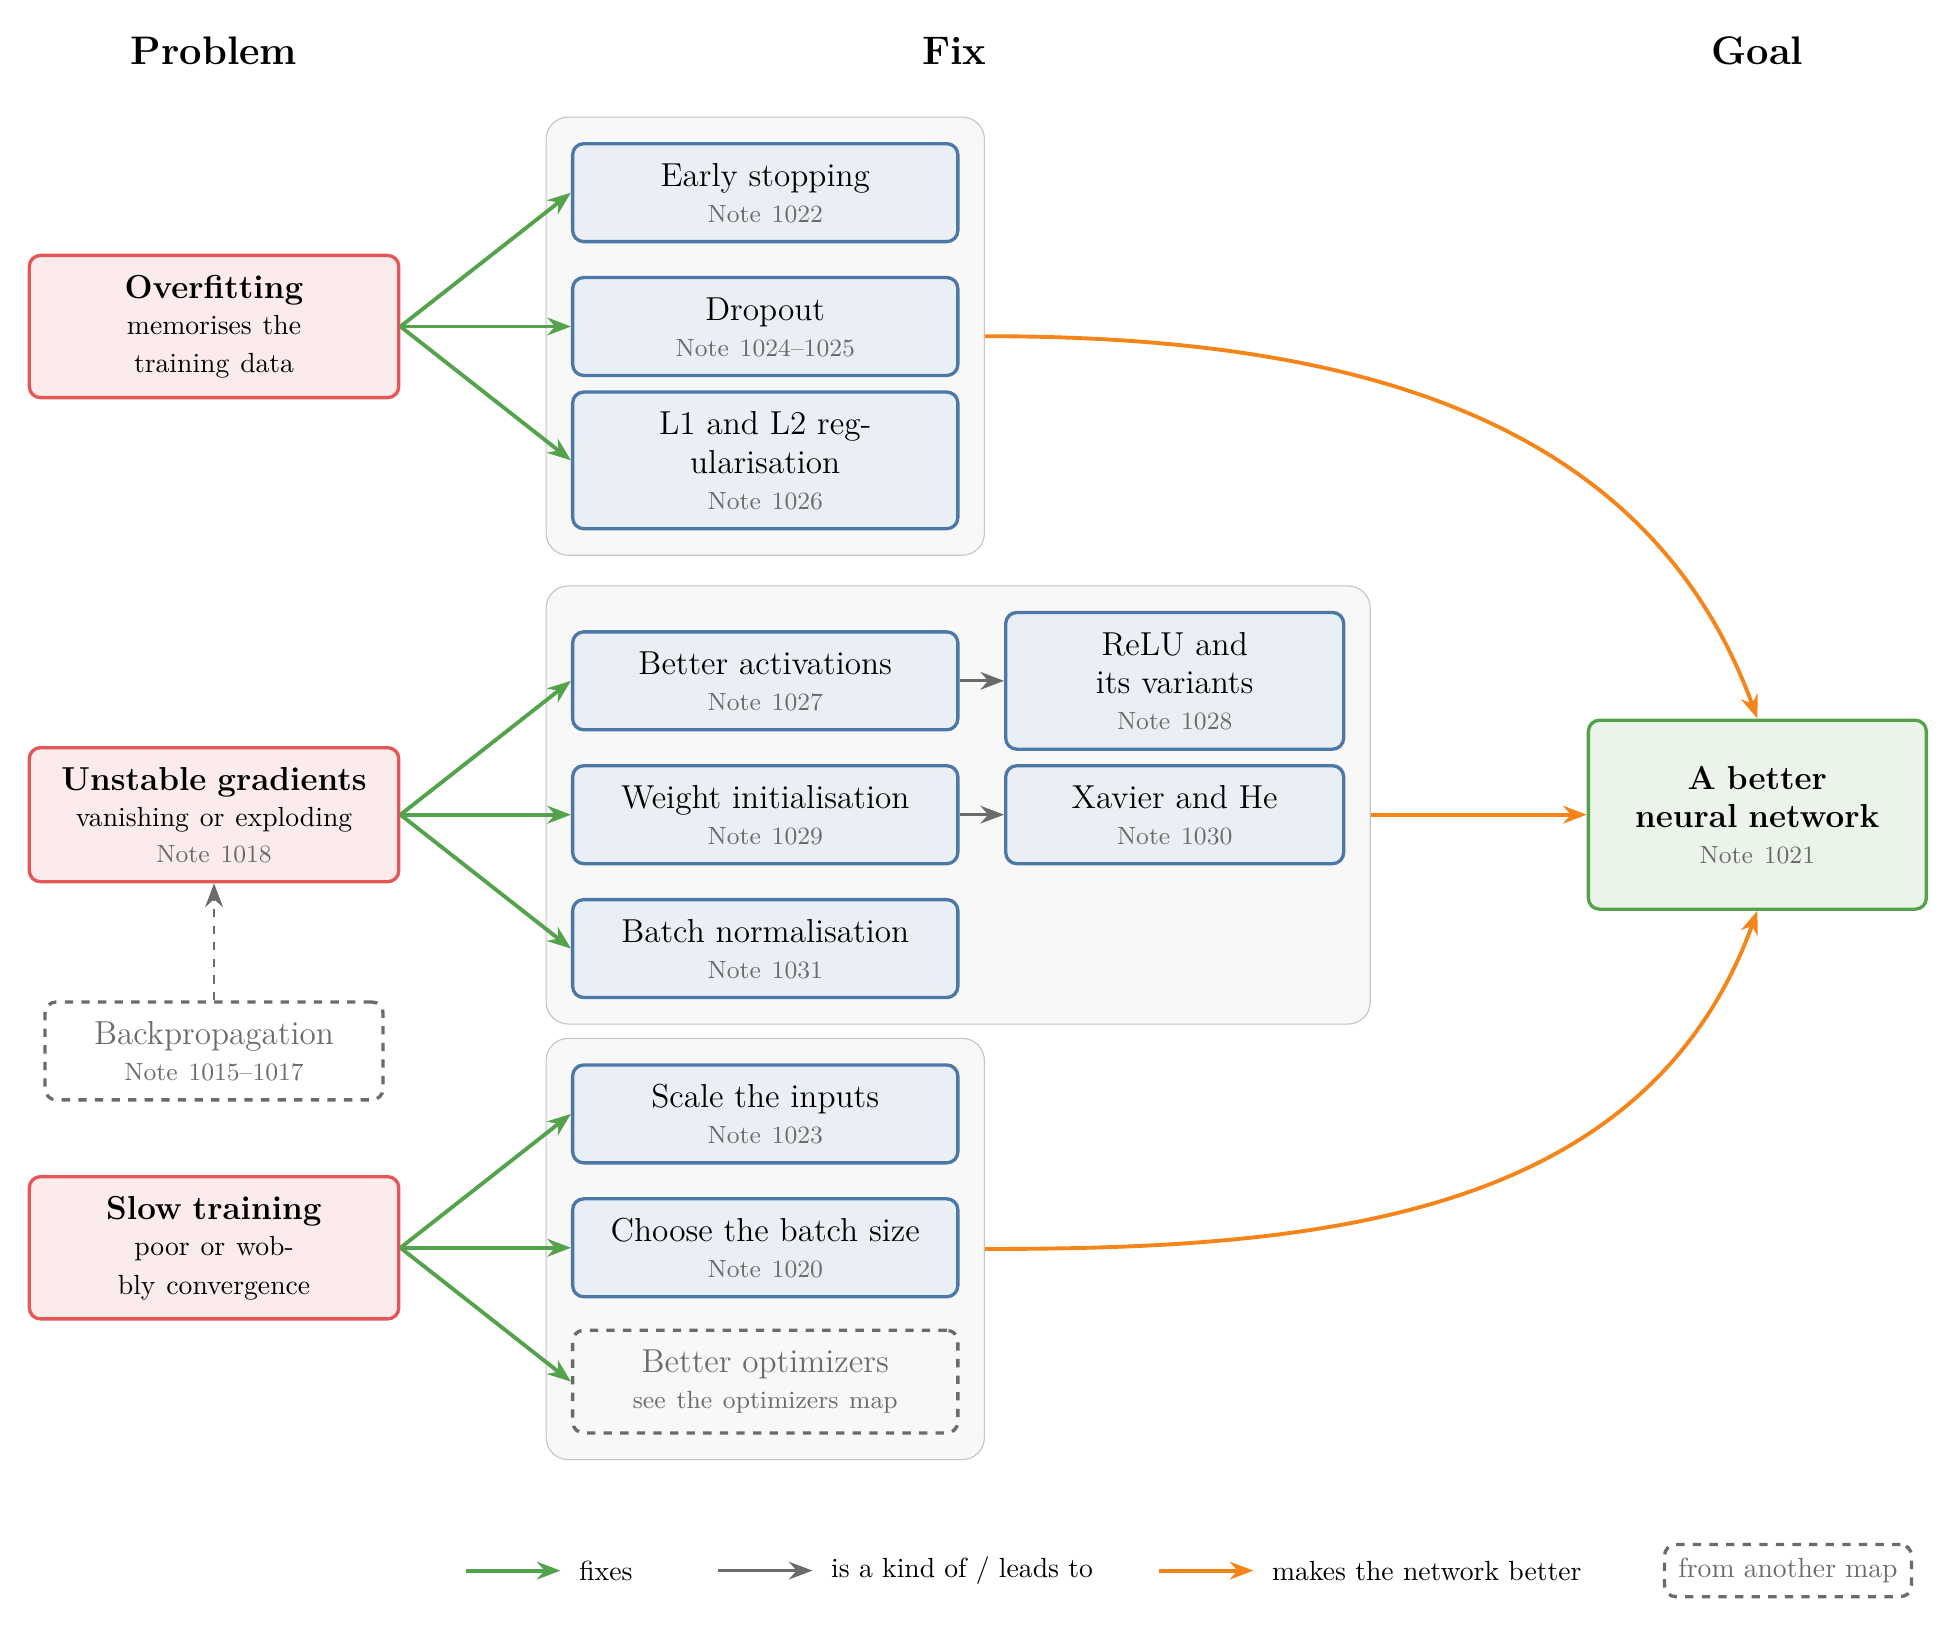
\begin{tikzpicture}[
    every node/.append style={font=\sffamily\large},
    prob/.style={box=cred, text width=4.2cm},
    fix/.style={box=cblue, text width=4.4cm},
    sub/.style={box=cblue, text width=3.8cm},
    prev/.style={draw=cgrey, dashed, rounded corners=4pt, align=center, inner sep=7pt, text=cgrey, text width=3.8cm, minimum height=1.1cm},
    group/.style={draw=cgrey!40, fill=cgrey!5, rounded corners=8pt, inner sep=9pt},
    fixes/.style={arrow, draw=cgreen},
    kind/.style={arrow, draw=cgrey, line width=1pt},
    goes/.style={arrow, draw=corange},
  ]
  \newcommand{\nt}[1]{\\[-1pt]{\small\color{cgrey}Note #1}}
  \node[title] at (0,9.9) {Problem};
  \node[title] at (9.4,9.9) {Fix};
  \node[title] at (19.6,9.9) {Goal};

  % problems
  \node[prob] (over) at (0,6.4)   {\textbf{Overfitting}\\[-1pt]{\normalsize memorises the training data}};
  \node[prob] (grad) at (0,0.2)  {\textbf{Unstable gradients}\\[-1pt]{\normalsize vanishing or exploding}\nt{1018}};
  \node[prob] (slow) at (0,-5.3) {\textbf{Slow training}\\[-1pt]{\normalsize poor or wobbly convergence}};
  \node[prev] (bp) at (0,-2.8) {Backpropagation\nt{1015--1017}};
  \draw[kind, dashed] (bp) -- (grad);

  % fixes: overfitting
  \node[fix] (es)  at (7,8.1) {Early stopping\nt{1022}};
  \node[fix] (do)  at (7,6.4) {Dropout\nt{1024--1025}};
  \node[fix] (reg) at (7,4.7) {L1 and L2 regularisation\nt{1026}};
  % fixes: unstable gradients
  \node[fix] (act)  at (7,1.9)  {Better activations\nt{1027}};
  \node[sub] (relu) at (12.2,1.9) {ReLU and its variants\nt{1028}};
  \node[fix] (init) at (7,0.2)  {Weight initialisation\nt{1029}};
  \node[sub] (xav)  at (12.2,0.2) {Xavier and He\nt{1030}};
  \node[fix] (bn)   at (7,-1.5) {Batch normalisation\nt{1031}};
  % fixes: slow training
  \node[fix] (sc)  at (7,-3.6) {Scale the inputs\nt{1023}};
  \node[fix] (bs)  at (7,-5.3) {Choose the batch size\nt{1020}};
  \node[prev, text width=4.4cm] (opt) at (7,-7.0) {Better optimizers\\[-1pt]{\small see the optimizers map}};

  % one panel per problem, one arrow per panel to the goal
  \begin{scope}[on background layer]
    \node[group, fit=(es) (do) (reg)] (g1) {};
    \node[group, fit=(act) (relu) (init) (xav) (bn)] (g2) {};
    \node[group, fit=(sc) (bs) (opt)] (g3) {};
  \end{scope}
  \foreach \f in {es, do, reg} \draw[fixes] (over.east) -- (\f.west);
  \foreach \f in {act, init, bn} \draw[fixes] (grad.east) -- (\f.west);
  \foreach \f in {sc, bs} \draw[fixes] (slow.east) -- (\f.west);
  \draw[fixes] (slow.east) -- (opt.west);
  \draw[kind] (act) -- (relu);
  \draw[kind] (init) -- (xav);

  \node[box=cgreen, text width=3.8cm, minimum height=2.4cm] (goal) at (19.6,0.2) {\textbf{A better}\\\textbf{neural network}\nt{1021}};
  \draw[goes] (g1.east) to[out=0, in=110] (goal.north);
  \draw[goes] (g2.east |- goal) -- (goal.west);
  \draw[goes] (g3.east) to[out=0, in=250] (goal.south);

  % legend
  \begin{scope}[shift={(3.2,-9.4)}, every node/.style={font=\sffamily, anchor=west}]
    \draw[fixes] (0,0) -- (1.2,0);           \node at (1.3,0) {fixes};
    \draw[kind] (3.2,0) -- (4.4,0);           \node at (4.5,0) {is a kind of / leads to};
    \draw[goes] (8.8,0) -- (10,0);            \node at (10.1,0) {makes the network better};
    \node[draw=cgrey, dashed, rounded corners=4pt, inner sep=5pt, text=cgrey, anchor=west] at (15.2,0) {from another map};
  \end{scope}
\end{tikzpicture}
\end{document}
